



\section{Ecuación de Michaels-Menten}

\marginpar{
\begin{minipage}{\marginparwidth}
    \begin{figure}[H]
        \centering
        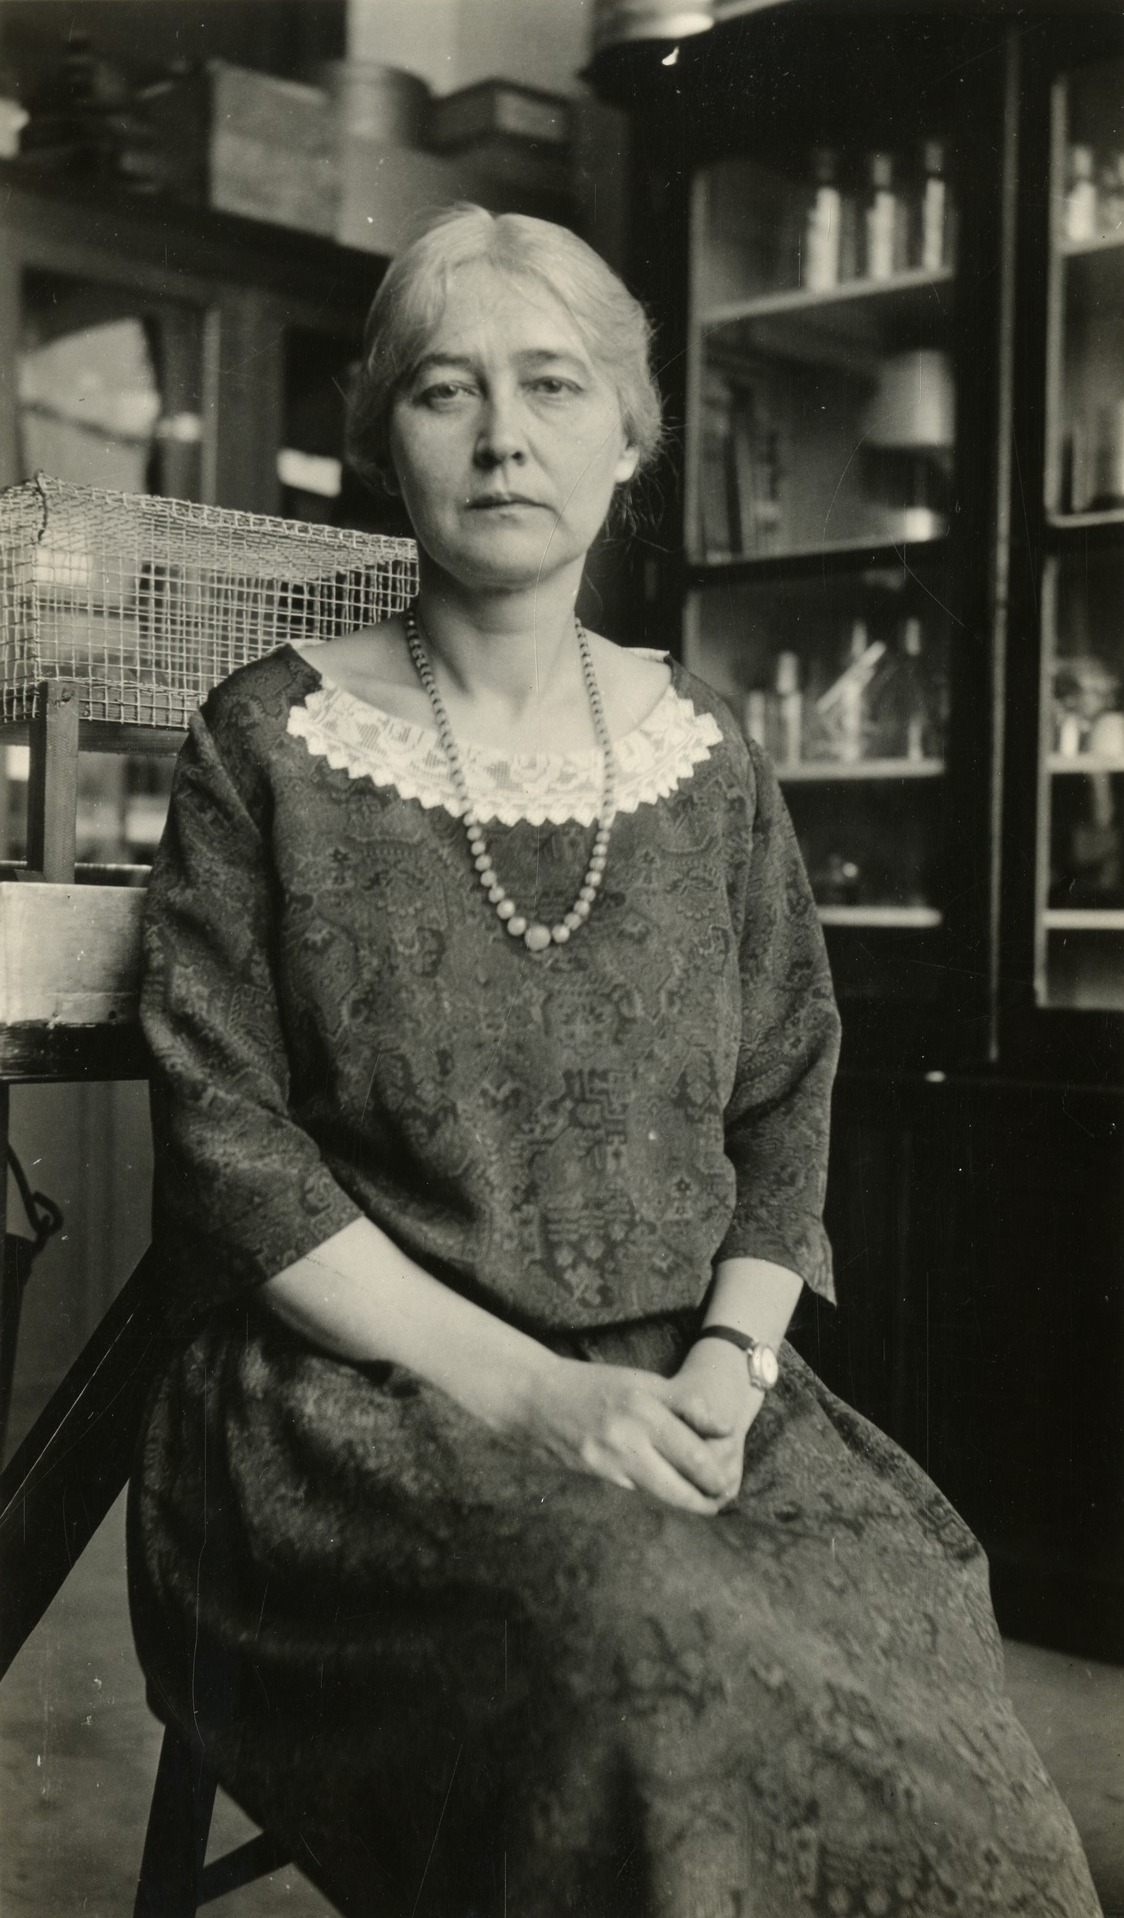
\includegraphics[width=\marginparwidth]{images/fig:leonora_menten}
        \rule{\marginparwidth}{0.2pt}
        \caption{Retrato de Leonora Menten}
        \label{fig:leonora_menten}
    \end{figure}
    \begin{figure}[H]
        \centering
        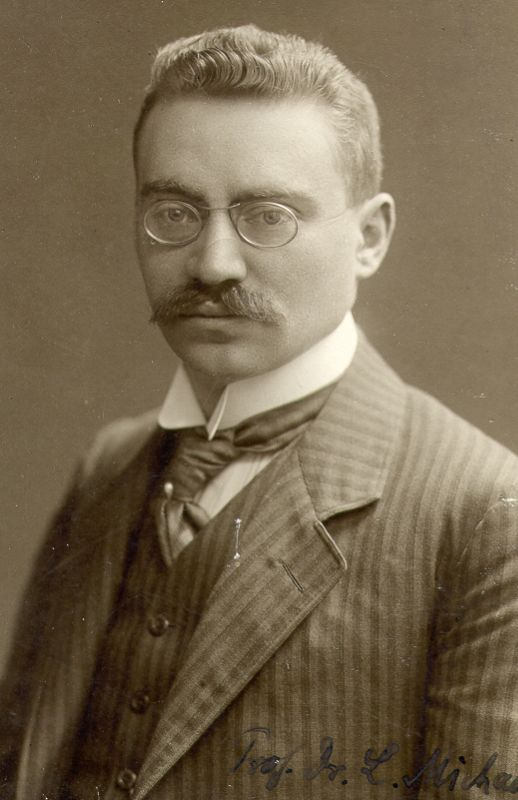
\includegraphics[width=\marginparwidth]{images/fig:leonor_michaelis}
        \rule{\marginparwidth}{0.2pt}
        \caption{Retrato de Leonor Michaelis}
        \label{fig:leonor_michaelis}
    \end{figure}
\end{minipage}
}

\begin{equation}
    v = \frac{V_{max}[S]}{K_{m} + [S]}
\end{equation}

Donde

\begin{equation*}
    Km = \text{[S] para alcanzar } \ \frac{1}{2}V_{max}
\end{equation*}

El valor de $K_{m}$ en la ecuación de Micahels-Menten es el conjunto de $K_{m}$ y $K_{cat}$

Determinar $V_{Max}$ y $K_{m}$ mediante una gráfica que tenga como ejes $[S]$ y $V$ es díficil, por lo que lo que se transforman los datos para que se pueda graficar una linea recta a partir de la cual, ahora sí, se puedan determinar los parámetros cinéticos ($V_{Max}$ y $K_{m}$) más facilmente.

Para los temas de linearización hay que primero recordar la ecuación de la recta y la forma de obtener $m$

\section{Ecuación de la recta y valor de $\mathbf{m}$}

\begin{align*}
    y &= mx+b
    \\
    m &= \frac{y_{1} - y_{0}}{x_{1} - x_{0}}
\end{align*}

Existen diferentes métodos por los cuales realizar esta transformación

\section{Valores de $\mathbf{m}$ y $\mathbf{b}$ en cada método}

Los diferentes métodos de linearización reemplazan los valores de $m$ y $b$ por ciertos parámetros cinéticos u operaciones con estos parámetros.

A su vez, es posible usar tales ecuaciones nuevas para obtener $V_{Max}$ y $K_{m}$, esto despejando la ecuación. La forma de despejarla dependerá de la formula usada, del parámetro buscado y de los datos con que ya se cuente.

En la siguiente tabla se recopila los valores que $m$ y $b$ adquieren en cada método, así como con $V_{Max}$ y $K_{m}$

    \begin{table}
\centering

\caption{Valores de $m$, $b$, $V_\text{Max}$ y $K_\text{m}$ en cada método de linearización}
\label{tab:valores_métodos_linearización}

{\small\setstretch{2}\rowcolors{1}{White}{Grey}

\begin{tabular}{M{0.275\linewidth}M{0.125\linewidth}M{0.125\linewidth}M{0.1\linewidth}M{0.15\linewidth}}\hline

    \theader{Método de linearización} & \theader{$\mathbf{m}$} & \theader{$\mathbf{b}$} & \theader{$V_\text{Max}$} & \theader{$K_\text{m}$} \\ \hline
    
    Lieneawever-Burk & $\frac{K_\text{m}}{V_\text{Max}}$ & $\frac{1}{V_\text{Max}}$          & $\frac{1}{b}$ & $V_\text{Max} \cdot m$   \\
    Eadie-Hosfstee   & K\sub{m}                          & $V_\text{Max}$                    & $b$           & $m$                           \\
    Hanes            & $\frac{1}{V_\text{Max}}$          & $\frac{K_\text{m}}{V_\text{Max}}$ & $\frac{1}{m}$ & $V_\text{Max} \cdot b$ \\
    
    \hline

\end{tabular}}\end{table}

\section{Métodos de linearización}

Aquí se desglosa en cada método cómo se cambian los valores en la ecuación de la recta por parámetros cinéticos, y cuales corresponden a cada uno.

\subsection{Lieneawever-Burk (Recíprocos)}

\begin{align*}
    y &= mx+b
    \\
    \frac{1}{V} &= \frac{K_{m}}{V_{Max}} * \frac{1}{[S]} + \frac{1}{V_{Max}}
    \\
    \\
    x = \frac{1}{[S]} \ &; \ y = \frac{1}{V}
    \\
    m &= \frac{K_{m}}{V_{Max}}
    \\
    b &= \frac{1}{V_{Max]}}
    \\
    \\
    V_{Max} &= \frac{1}{b}
    \\
    K_{m} &= m * V_{Max}
\end{align*}

\subsection{Eadie-Hosfstee}

\begin{align*}
    y &= b - mx
    \\
    V  &= V_{Max} - K_{m} * \frac{V}{[S]}
    \\
    \\
    x = \frac{V}{[S]} \ &; \ y = V
    \\
    m &= K_{m}
    \\
    b &= V_{Max}
    \\
    \\
    V_{Max} &= b
    \\
    K_{m} &= m
\end{align*}

\subsection{Hanes}

\begin{align*}
    y &= xm+b
    \\
    \frac{[S]}{V}  &= [S] * \frac{1}{V_{Max}} + \frac{K_{m}}{V_{Max}}
    \\
    \\
    x = [S] \ &; \ y = \frac{[S]}{V}
    \\
    m &= \frac{1}{V_{Max}}
    \\
    b &= \frac{K_{m}}{V_{Max]}}
    \\
    \\
    V_{Max} &= \frac{1}{m}
    \\
    K_{m} &= V_{Max} * b
\end{align*}

